\documentclass[isoft]{poster_class_UofC}

\usepackage{lipsum}
\usepackage{natbib}
\usepackage{booktabs}
\usepackage{subfig} 
\usepackage{amsmath} 
\usepackage{textcomp} 
\usepackage{url}  
\usepackage{hyperref}
\usepackage[utf8]{inputenc}
\usepackage[english]{babel}

%%%%%%%%%%%%%%%%%%%%%%%%%%%%%%%%%%%%%%%%%
%%               Configs               %%
%%%%%%%%%%%%%%%%%%%%%%%%%%%%%%%%%%%%%%%%%

% Choose one of the section color {ufglhblue | ufgdkblue | dkblue | black | gold}
\setsectioncolor{red} 
\setsubsectioncolor{gold}

% Define width of the rule or hide it by setting 0pt or commenting the command 
%\setcolumnseprule{2pt}

% Inform the paths to the logo files or leave empty one or both parameters. 
% There are three options [ T | M | B ] to positioning them.
%\setlogos[T]{images/uc-vert-rgb}

% Choose one of the background options {1 | 2 | 3}. 
% Actually, one can select any graphic file in backgrounds directory. 
\setbackground{1}

% Resize the title to keep it in two lines 
\settitlesize{68pt}{64pt}

% General info
\title{\uppercase{U-turning on Deep Learning Methods for Cell Counting:\\ A Bayesian Regression Approach}} 

\author{Andrew Pohl\textsuperscript{1}, Dylan Loader\textsuperscript{2}, Mingkuan Wu\textsuperscript{2}, Daniel Yang\textsuperscript{2}} 

\department{\textsuperscript{1}Faculty of Kinesiology. \textsuperscript{2}Department of Mathematics and Statistics \\ 
University of Calgary}

\email{ \text{andrew.pohl@ucalgary.ca, dylan.loader@ucalgary.ca, mingkuan.wu@ucalgary.ca, daniel.yang@ucalgary.ca} }

%\class{Projeto Ciência no Parque}

\posteryear{2019}

\copyrightholder{Department of Mathematics and Statistics - University of Calgary}

%%%%%%%%%%%%%%%%%%%%%%%%%%%%%%%%%%%%%%%%%
%%           End configs               %%
%%%%%%%%%%%%%%%%%%%%%%%%%%%%%%%%%%%%%%%%%

\pagestyle{fancy}
\begin{document}
    \begin{poster}
    
    %%%%%%%%%%%%%%%%%%%%%%%%%%%%%%%%%%%%%%%%%
    %%             Begin poster            %%
    %%%%%%%%%%%%%%%%%%%%%%%%%%%%%%%%%%%%%%%%%
    \section{Introduction}
With the invention of high throughput automated image cytometry techniques, the generation of cellular microscopy image data has accelerated drastically and automated methods are required to count cells.  \\

 Current methods for cell counting are often adversely affected by deviations in image focus, by the use of differing cell staining techniques and by the fact that cells often overlap each other in images. \\

 Given the recent success of deep learning image processing methods such as the U-Net neural network \cite{FalkThorsten2019Udlf}, we hypothesise that prediction models for cell count will improve when images are pre-processed by a U-Net neural network.


        
    \section{Methods}%
        
        \subsection{Dataset}
 The dataset consists of 3600 simulated fluorescence microscope slides obtained using 2 types of stain and 3 levels of imaging blurring, with cell counts ranging from 1 to 100 \cite{VebjornLjosa2012Ahmi}.\\

 The dataset was segmented into three separate sets.  A testing set of $1200$ images was with-held by the judges.  To construct a robust training and validation environment we further segmented the training set into training (1920 images) and validation sets (480 images).

             \subsection{Prediction Models}    
  A Bayesian implementation of polynomial regression was applied to predict the number of cells from either a raw image or U-Net generated image mask.  \\

 It was assumed that the cell count followed a rounded, truncated $[0,1]$ normal distribution such that: $y_{i,j,k} \sim N(\mu_{i,j,k}, \sigma^2)$. \\

 To account for increased cell overlap (and consequently fewer pixels per cell) as the number of cells per image increased, the sum of the normalised pixels $x$ for each image $i$ belonging to stain $j = 1,2$ and blurring level $k=1,2,3$, along with its square were used as covariates to estimate the corresponding cell count ($y_{i,j,k}$).\\

 Regression coefficients $\beta_1, \beta_2$ and$\beta_3$ were allowed to vary on three levels: 
\begin{adjustwidth}{2cm}{}
\begin{enumerate}
 \item Single level where regression coefficents were not allowed to vary regardless of stain/blur group.
 \item A varying slope model where $\beta_2 $ and$\beta_3$ were allowed to vary based on stain/blur group.
 \item A varying slope and intercepts model where all coefficients were allowed to vary given the corresponding stain/blur group.
\end{enumerate} 
\end{adjustwidth}
     

        \subsection{U-Net Image Preprocessing}
 A 10 layer encoder-decoder U-Net simplified from the architecture provided by 
Falk et al. (2019) \cite{FalkThorsten2019Udlf} was trained on a subset of 830 images wtih ground-truth segmentation masks \cite{VebjornLjosa2012Ahmi}.

                \vspace{1cm}
        \begin{figure}
                    \centering
            \captionsetup{type=figure}
            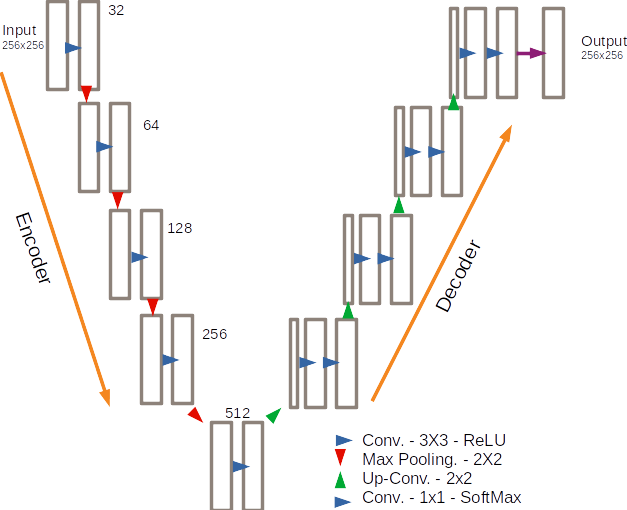
\includegraphics[scale=1]{./images/UNet_Arch.png}
            \caption{U-Net architecture used for image segmentation.}
            \label{fig:U-NET}
        \end{figure}
              \vspace{1cm}
              
 To increase the training set size (and improve image segmentation performance) a data-generator was constructed which rescaled images to 256x256 pixels and performed random rotations along with horizontal and vertical image shifts.


        \section{Results}%
 RMSE on the with-held validation set reduces with each layer of complexity with the most complex varying slope and intercept model producing the most accurate predictions. \\

 The leave one out information criteria \cite{VehtariAki2017PBme} does not increase with increasing model complexity suggesting the model is not over-fit to the training data. \\

 Contradictory to our hypothesis RMSE is similar between raw images and when image preprocessing via U-Net was implemented suggesting no improvement in prediction when using RMSE.

                \vspace{4cm}
            \begin{table}
                \centering
                \captionsetup{type=table}
                \setlength{\tabcolsep}{20pt}
                \caption{Performance of regression models on training and validation data set}
                \label{tab:Results}
                %\renewcommand{\arraystretch}{1.2}
                \resizebox{0.5\textwidth}{!}{%
                \begin{tabular}{l|c|cc|cc}
				\hlinewd{3pt}
                \multirow{2}{*}{Model} & Number of & \multicolumn{2}{c}{Raw Images} & \multicolumn{2}{c}{U-Net}\\
                & Parameters & RMSE & PSIS-LOO & RMSE & PSIS-LOO \\
                \hline
                1: $\mu_{ijk} = {\beta_0} + {\beta_1} x_{ijk} + {\beta_2} x_{ijk}^2$ & 3 & 21.77 & 19265.0 (28.7) & 19.80 & 18244.8 35.9\\
                2: $\mu_{ijk} = {\beta_0} + {\beta_1}_{jk} x_{ijk} + {\beta_2}_{jk} x_{ijk}^2$ & 13 & 12.45 & 17568.8 (175.3) & 13.39 & 16551.7 (106.3)\\
                3: $\mu_{ijk} = {\beta_0}_{jk} + {\beta_1}_{jk} x_{ijk} + {\beta_2}_{jk} x_{ijk}^2$ & 18 & 1.74 &  7572.2 (98.2) & 1.94 & 8125.9 (112.2)\\
                \hlinewd{3pt} 
                \end{tabular}
            }
            \end{table}
            \vspace{1cm}
            
 U-Net segmentation had the effect of making differences between the 3 levels of blurring and two different stains become more apparent. \\

             \vspace{1cm}
           \begin{figure}
            \centering
            \captionsetup{type=figure}
            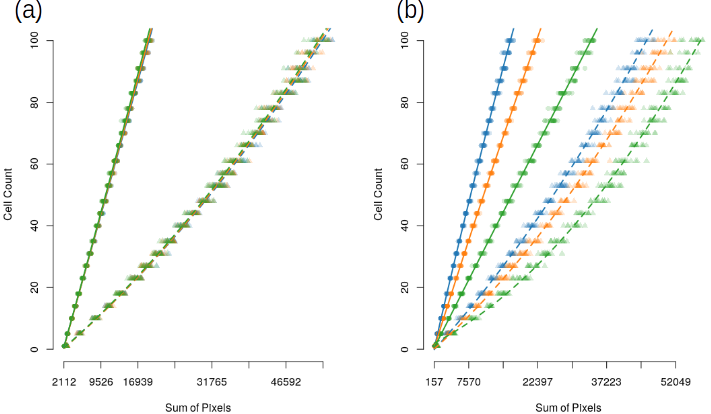
\includegraphics[scale=1.7]{./images/rawVUnet.png}
            \caption{Relationship between sum of pixels and cell count for (a) raw images and (b) images after U-Net segmentation processing. Low blur is indicated in blue, medium in orange and high in green with nuclei stained images represented by circles and cell body stain represented by triangles. Fitted regression lines for the varying slopes and intercept model are included.}
            \label{fig:Results}
        \end{figure}   
            \vspace{1cm}
 With Bayesian mixed level regression models we are able to sample from the posterior predictive distribution for the number of cells given each image in the test set and generate prediction intervals. The prediction intervals for images within the validation set were well calibrated with 95.8\% of 95\% prediction intervals containing the true cell count and intervals having an average width of 6 cells.



             \vspace{1cm}
           \begin{figure}
            \centering
            \captionsetup{type=figure}
            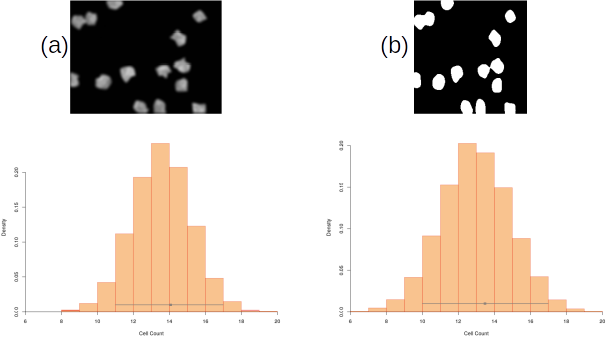
\includegraphics[scale=1.7]{./images/PostPredDist.png}
            \caption{Posterior predictive distribution for an image containing 14 cells when generated via the raw image (a) or U-Net segmentation mask (b).}
            \label{fig:PostPredDist}
        \end{figure}   
            \vspace{1cm}
            
    
        \section{Conclusions}
 A multilevel polynomial regression model was effective in providing fairly accurate estimates of cell count and well calibrated prediction images with low computational cost while maintaining parameter imperturbability. \\

 There was no apparent benefit to applying a segmentation mask generated by a U-Net Neural Network with regards to improving prediction performance.
  
        \section{Acknowledgements}
We would like to thank Dr. Matthew Greenberg for his invaluable insights in guiding this work.  

        \bibliographystyle{abbrv}
        \bibliography{refs}
    
    %%%%%%%%%%%%%%%%%%%%%%%%%%%%%%%%%%%%%%%%%
    %%               End poster            %%
    %%%%%%%%%%%%%%%%%%%%%%%%%%%%%%%%%%%%%%%%%
    
    \end{poster}

\end{document}

 
